\chapter{Related Work and Table of Profiles}
\label{chapter2}

In the first part of the chapter, we will review the existing work done and show possible use-cases for the load profiles.  
In the second part of the chapter most commonly used LP features will be presented. 
Using them, a table of profiles will be built. 
The table will be populated using the publications from the first part of the chapter.
This will enable us an overview of existing work, and expose possible missing gaps in scientific research.

\section{Related Work}
\label{sec:related_work}
Work that is related to load profiling can be found in two research verticals. 
The first one is load profiling and LP models, in most cases study the LP curve of a building or appliance.
The second vertical is anomaly detection in energy consumption data. There are quite a few connections between the two. 
For example, if one wants to do anomaly detection, one must first build some kind of "normal consumption profile", in other words, an LP.

\subsection{Load Profiling}

One of the first publications on load profiling was published by Train et al.\cite{TRAIN19851103}.
They used a bottom-up approach using sub-meter data and other socioeconomic and demographic characteristics 
to create an LP or statistically adjusted engineering (SAE) as they call it.
They can adjust the curve based on weather, dwelling size, and income. 
In the same year, Walker et al.\cite{WALKER1985} published a paper where they used a bottom-up approach with psychological factors to create probability models of when will an individual use an appliance.
Since then there were two more in 1995. Research picked up the pace in 2005 with 7 publications in 2013 as Figure \ref{fig:Distribution} shows.

\begin{figure}[H]
	\centering
	\caption{Distribution of publications on load profiling from 1985 to 2020. The graph was published by \protect\cite{Review2021}.}
	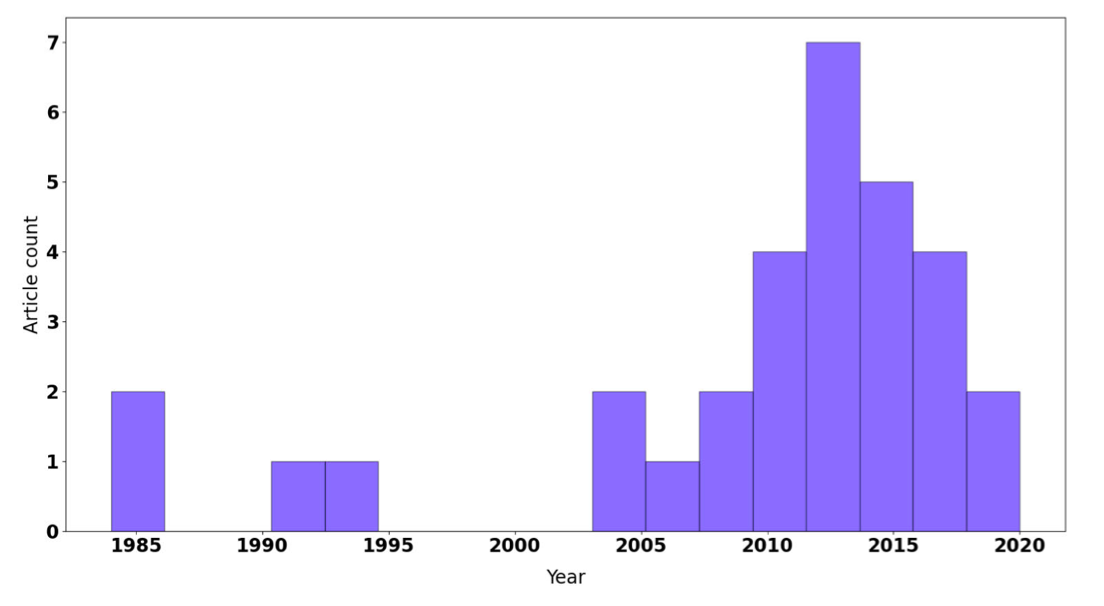
\includegraphics[width=0.9\textwidth]{Figures/publications.png}
	\label{fig:Distribution}
\end{figure}

Load profiling can be performed in two ways: bottom-up and top-down. 
A bottom-up approach as authors in \cite{SWAN20091819} state "calculates the individual dwelling energy or electricity consumption and extrapolates these results over a target area or region"
Whereas with top-down approach as authors in \cite{SWAN20091819} state "uses the total energy or electricity consumption estimates to assign them to the characteristics of the building stock"
In other more general words, bottom-up uses sub-meter data, Top-down uses aggregated data. 
In our case, we take a deeper dive into the bottom-up approach.

The author in \cite{Review2021} did a comprehensive review on load profiling. The author defined various load-profile application
subgroups such as demand-side management, planning and control design of energy systems, and residential LPs. The author also 
grouped modeling techniques as probabilistic models, Markov chains, and Monte Carlo. The author first disclosed the current state of load profiling and issues with past work.
They made a review of existing load profiling models
and asses the-state-of-the art. 
Next, they pointed out future research directions
and applications of load profiling models. Finally, the author exposes issues that researchers face and addresses possible solutions with conclusions.

Gerbec et al.\cite{GERBEC2005} tried to assign typical LPs to a particular group of consumers based on their activity. 
To achieve that, they used probabilistic neural networks as a way of classification. Their methodology was tested in real-use scenarios. 

Gao et al.\cite{Gao2018} makes use of the bottom-up method to build a forecasting framework for household
load profiling, which takes into account the consumption patterns of residents. 
A model falls into the demand response use case.
They have developed a "single-day extraction model", designed to select the same days by comparing environmental and household factors, which influence energy consumption.
By using this approach, they have improved the accuracy of predicting the behavioral patterns of dwellers. 
Results show that their method successfully modeled daily usage.

Chuan et al.\cite{Chuan2014} uses load profiling to optimize energy consumption distribution during the day.
This reduces peak usage and alleviates load off the grid. The author used the bottom-up method, that is, using sub-meter data.
Using this data, they made daily usage analyses on a one-hour basis. Using this information they optimized the daily activation of appliances
so that peak usage was not as high. Results show that peak shedding was successful. 

Csoknyai et al.\cite{Csoknyai2019} analyzes energy consumption patterns and intervention strategies in residential buildings.
Authors achieve this using a "serious game approach" with a combination of direct user feedback using smart meters. 
The application also provides advice, comparisons, savings, reduction goals, and monitoring.
The approach takes into account almost all dimensions of residential energy usage. Their results show that their serious game was not
able to induce energy-saving behavior.

Jeong et al.\cite{Jeong2021} used extreme points in the appliance usage curve to cluster usage profiles.
Usually, the first usage peak is in the morning, and the second one is in the evening. 
Additionally, they used demographic characteristics that are: region, area, age, salary, etc. to improve the results.
Using collected data, they clustered profiles. They discovered 6 different usage profiles, 
where every cluster had a physical meaning such as energy-saving, morning heavy, evening heavy, etc.

Another clustering methodology was proposed by Park et al.\cite{Park2019}, using load image profiles and image processing.
They represented time series data as an image. The image is a grid of squares where the y-axis contains monthly data with a resolution of one day,
x-axis contains daily data with a resolution of one hour. Grid is color filled with an algorithm that authors developed,
where red means more activity and blue less. Using digital image filters they transformed the type-1 image to type-2 and from there
used a threshold to obtain type-3. Using that information they clustered data based on images similarly. They used three different 
clustering methods: k-means, FCM, and EM algorithm. Using the Davies-Bouldin index, they were able to prove that image-based clustering performs better than non-image.

Abreu et al.\cite{Joana2012} clustered different LPs using electricity consumption data and surveys using data from residential homes.
They used PCA and k-means resulting in 5 clusters. Similar to other load profiling papers. 

Whereas most of the above-mentioned papers focused on aggregated consumption of building to build an LP,
authors \cite{Issi2018} focused on appliance-level load profiling.
Their main contribution was to create a realistic per-appliance LP.
They developed a wireless measurement system with smart plugs that enabled them to obtain power signatures for each appliance. 
They evaluated the data and based on observations they determined working cycles for each appliance.
Furthermore, they concluded that 15 \% of consumed power can be shifted, where they took tariffs into account. 

\subsection{Anomaly Detection in Building Energy Consumption Data}

A review on anomaly detection in building energy consumption data was written by authors \cite{HIMEUR2021116601}.
Here, the authors took a deep dive into detecting anomalies in energy consumption in buildings. 
The author first makes an overview of existing anomaly detection schemes and applications.
Second, they perform a critical analysis and an in-depth discussion of the state-of-the-art.
Next, they describe current trends such as NILM anomaly detection. Finally, they assemble a set of future research directions. 
Both reviews pointed out that NILM anomaly detection or NILM load profiling is a possible future research direction.

Rashid et al.\cite{NILMAD2019} propose an algorithm
that functions on top of existing state-of-the-art NILM algorithms Hidden Markov model,
combinatorial optimization, Latent Bayesian Modeling, and Graph-based Signal Processing.
They focus on three appliances, a fridge, freezer, and heater. Their metric was the number of operation cycles and energy used within those cycles. 
They implemented sigma variables to represent standard deviation and used rule-based anomaly detection.
So if energy or counts are significantly larger than the mean then the day is considered anomalous.
Their rule had only one manual setting and that was a number of standard deviations before the sample was considered anomalous.
Their results show that sub-meter anomaly detection works decently whereas NILM-based anomaly does not work at all. 

The same author published another paper \cite{NILMAD22019} in the same year, where they took a similar approach, except that they used 
only compressor-based appliances such as fridges and air conditioners. They also added a rule to their existing rule-based anomaly 
detection algorithm, but the results still showed that NILM algorithms are not there yet. 

Castangia et al.\cite{Castangia2021} used disaggregated sub-meter data to detect anomalies in use consumption.
They used a private dataset of 20 homes from northern Italy with no synthetic anomalies. 
The dataset included data from 2018 to 2020 meaning it included covid-induced anomalies. 
The authors first pre-processed the data by aggregating input load in hourly energy consumption, 
the second derived additional features, which are the time of use and duration of the activation.
They use that data to detect single-point deviations for which they implemented the isolation Forest algorithm and
anomalous trends for which to detect, they implemented Change Point Detection. 

\section{Use-cases}
\label{sec:use-cases}

The general classification of use-cases was done in Section \ref{sec:use_cases_tree}. 
Here, we will focus on presenting these use-cases in great detail.
This will be achieved by analyzing the use-case publications and in some cases providing additional solutions.

\subsection{Grid Management}
\label{sec:grid_managment}
\subsubsection{Zero Energy Buildings and Energy Saving}

As mentioned before many applications for load profiling could be used to reduce energy use and increase energy efficiency. 
With the emerging EV-market and ever-increasing installation of heat pumps, more and more energy is being used in form of electricity. 
This means, that most of the current power grids would have to be upgraded to keep up with demand.

On the other side, more and more photovoltaic systems are being installed,
which is slowly shifting energy production towards end-users.
Slowly energy grid is starting to shift towards so-called distributed energy resources or "DER" \cite{MORENOJARAMILLO2021445}.
DERs include all kinds of micro-energy sources such as PV, wind power, water power, and all kinds of energy accumulators that can store 
and release energy when needed such as heat pumps with hot water storage, home batteries, and EVs that can be used as a battery.

With smart management, these appliances could be used in a way that would reduce the net flow of energy and alleviate the load off the power grid.
A way to achieve this is via load profiling and load modeling. 
To manage the appliances, a control system would have to be put in place \cite{DirectLoadControll2021}.
It would be enough to control a few appliances that consume most of the energy. 

Since consumers take part in producing the energy, they are often called "prosumers" \cite{Prosumer2016}.
They will be an essential part of the European Union's plan to reach zero-energy buildings
and near-zero-energy buildings \cite{eu2021}. The directive was accepted in 2010 and was recast in 2021.
The plan is set to be realized in the next decade.

An actual use-case would be an EV owner with an installed PV system and heat pump, who works from home on occasion.
In this case, two profiles would be developed. Normal workday and work-from-home day.
Additional information would be obtained from the user's calendar. 
On a normal workday, the system would use PV energy to heat the water and store it, based on the user profile.
On work-from-home days, the system would start charging the car with the morning sun, using only the PV energy. 
In the evening hours, when consumption rises and production falls, EVs could inject the power back into the house. 
Again using appliance LPs to mitigate net energy flow as close to zero as possible (zero-energy building).
With the ever-increasing power capacity and increasing range of EVs, more and more battery capacity could be used for mitigation. 
In the case of grid batteries, similar steps could be taken.
This process is called vehicle-to-grid, and it is an important step towards zero-energy buildings \cite{EV2018} \cite{EV2020}.

One other way to use user LPs is to optimally distribute the load by studying user's usage patterns as \cite{Chuan2014} \cite{shift2015} proposed in their papers. 
This could be further extended to neighborhoods connected into peer 2 peer energy distribution networks.
As mentioned earlier, the way to save energy consumption is to distribute it as locally as possible. 
Knowing the usage patterns of all peers, the system could optimally distribute the energy using DERs across all homes without dwellers even noticing.

Another use-case could be using a heat pump and heat storage,
where besides the user's usage patterns system would also obtain weather forecasts from the internet.
Heat pumps that extract heat from the air are more efficient when temperature differences are smaller. 
The heat pump could store energy when warm and release the energy when cold.
Based on the user usage profile, energy could be optimally distributed.

Many papers have been published, where authors explored ways to reduce the energy consumption of users by studying user consumption patterns \cite{energy_saving3} \cite{energy_saving1} \cite{energy_saving4} \cite{energy_saving3}.
Energy saving is done through instant feedback, reduction goals, rewards, and by comparing their user profile to the average user as the authors did in paper \cite{Csoknyai2019}.
Source \cite{eu2006} states that as much as 20 \% of energy could be saved by managing consumption.

\subsubsection{Demand Response}

An increasing percentage of renewable resources is troubling energy distributors, due to the nature of renewable resources.
In the prior Chapter, it was mentioned how energy-saving measures would benefit users and their peers.
One other use-case would be cooperation between end-user and energy distribution companies.
Joint actions between them would benefit both as authors show in papers \cite{cooperation2008} \cite{cooperation2010}.

The electricity provider could control the main appliances so that load on the power grid is uniform,
with as few peaks and valleys as possible. For this to function, users would have to allow the installation of energy meters and controllers 
on appliances that use the most electricity \cite{gridDirectControll2015}. One way to achieve this is to control the voltage of loads \cite{controll2014} the other
way is to shift the loads in time \cite{shift2015}.
This process is called direct load control \cite{DirectLoadControll2021}, and it is part of demand response program \cite{DemandResponse2018}.

"DR program is a voluntary PJM program that compensates end-use (retail) customers for reducing their electricity use (load)
when requested by PJM during periods of high power prices, or when the reliability of the grid is threatened." \cite{DemandResponse2018}

The benefit to the user would be the lower cost of charging EVs and heating the building.
This is already done through so-called small and high tariffs.
More detailed user LPs would enable the electricity provider to introduce real-time tariffs.

The user would have three options. The first one would be that users can use the appliances as freely as they desire, this would result in a normal tariff.
The second option would be to use the appliances as regularly as possible, this would lead to lower tariffs.
The third option would be to leave the management of main appliances to the electricity provider via direct load control.
The provider would combine the user appliance LP and the real-time market price of energy to optimize the cost \cite{optimiseCostShift2015}.
This would lead to free or even negative prices of electricity since distribution companies have to keep the frequency of the grid as stable as possible.

For them to stabilize the frequency, they sometimes have to resort to load shedding.
Load shedding is a process where a load is disconnected from the grid to keep the grid in sync \cite{loadShedding2006}.
Commonly whole neighborhoods are being disconnected, affecting their daily lives.
Using user LPs, distribution companies could disconnect the load in a way that would minimally affect the end user. 
When they would need to load the grid due to low demand, they could charge EVs free of charge or even pay to do so. 
This benefits the company as well since they do not need to lower energy production, which can be expensive. 

\subsection{Anomaly Detection}

One use-case of anomaly detection was already mentioned in the Elderly care Chapter.
One more thing that could be detected, using load profiling, would be the altered operation of appliances.
In the case of a fridge, the system would detect that duty cycles are too long.
The increased duty cycle can be caused by cooling liquid leakage, the fridge being open or compressor motor malfunction.
Heat pumps work on the same basis as fridges, meaning the same anomalies could be detected. 
The malfunction could also be detected in heating element appliances such as toasters or boilers. 
Since mentioned appliances are one of the largest consumers in a household,
early enough detection could lead to large energy-saving benefits \cite{NILMAD2019}.

\subsubsection{Elderly Care}

The aging population is an increasing socioeconomic issue.
The elderly are facing many issues when staying at home alone for extended periods.
Accidents such as falls or the inability to do choirs due to health-related issues or even dementia-induced issues 
such as leaving appliances on for long periods could all be detected, using sub-meter data such as authors in publications \cite{elder1} \cite{elder2}
explore in their papers.

To detect falls or other issues a normal daily appliance use profile would be developed.
It would involve routine behavior of users such as turning on the coffee machine in the morning, the stove and oven at the noon or using the toaster in the evening.
All these routines could be measured and tracked. Using this data, a profile would be developed.
The probability of an anomaly and a threshold would enable the system to detect an issue.

An example would be: the coffee machine not turning on in the morning or the stove and kitchen vent not being used at the noon.
Another issue could be detected if the appliance would be used more frequently or for extended periods of time. 
This could indicate that the user forgot to turn off the stove, oven, or even a light. The same system could detect 
that a fridge or a freezer was left open since the duty cycles would be longer and more frequent. 
As soon as the issue would be detected it would notify the caregiver to check on the patient.

\subsection{Other}

Load profiling could also be used as feedback for the engineers and designers,
of how a device is being used and if it is being used as designed. 
This would enable the manufacturers to improve their products according to 
user's needs, without unnecessary features.

Yip et al.\cite{energyStealing2018} uses anomaly detection algorithms and load profiling to detect energy lost due to non-technical losses.
This occurs after the smart meter is exposed to cyber or mechanical attacks and its measurements are off. 

One other use-case could be occupancy detection of buildings such as the authors explore in paper \cite{occupancy2013}. Information about 
occupancy could be used as part of elderly care monitoring or in the case of building
automation, to run certain tasks when a user enters or leaves the room or a building.

\section{Table of Profiles}

% While in related work we examined load profiling in general,
% this section focuses on how data is presented with LPs.  
% It can be portrayed in various shapes and forms,
% using all kinds of attributes and features to do so. 

% First, main load profiling features will be defined.
% Second, using these features a general LP table will be constructed.
% Third, references from related work and use cases will be mapped to the table, from which main features will be selected.
% Fourth, using a reduced feature set a more detailed table will be formed.
% Again, the table will be populated using the same references as before.
% Finally, using this information a research direction will be formed.

In the first part of this Chapter, we focused on the general concept of load profiling and reviewed the existing literature on the topic.
In this second part, we will delve into the various ways in which load profiling data can be presented using LPs. 
We will begin by constructing a general LP table from previously defined features in Section \ref{ssec:feature_set}
Next, we will map the references and use cases from the related work reviewed in previous chapters to this table and select the main features to use.
Using this reduced set of features, we will create a more detailed LP table and populate it with information from the same references.
Finally, we will use this information to identify potential directions for future research in this field.

% Combining these features with  related work from Section \ref{sec:related_work} and use-case references from Section \ref{sec:use-cases},
% we can extract the most commonly used features to portray the LPs.

% \begin{outline}
%     \1 power
%     \1 time
%     \1 appliances (a set)
%     \1 operating time (how long appliance or appliances is turned on)
%     \1 number of activations (How many times appliance or appliances were turned on)
% \end{outline}

\subsection{General Table}
Using these features defined in Section \ref{ssec:feature_set} we can form a Table with all possible combinations.
Table \ref{tab:general_map} is then populated with references from previous chapters.
To understand the table more clearly, let's imagine that each feature is used as an axis label when plotting. 

\begin{table}[H]
    \centering
    \caption{General table of LPs}
    \label{tab:general_map}
    \begin{tabular}{|c|c|c|c|c|c|}
    \hline
        &
        \begin{tabular}[c]{@{}l@{}}power \end{tabular} &
        \begin{tabular}[c]{@{}l@{}}number of\\ activations \end{tabular} \\ \hline
        \begin{tabular}[c]{@{}c@{}}time\end{tabular}        & \multicolumn{1}{c|}{\begin{tabular}[c]{@{}c@{}} \citeyear*{Chuan2014}  \citeyear*{Csoknyai2019}  \citeyear*{H0} \\ \citeyear*{KAVOUSIAN2013184}  \citeyear*{WALKER1985}  	\citeyear*{GERBEC2005} \\ 	\citeyear*{Gao2018}  	\citeyear*{Jeong2021}  \citeyear*{Joana2012} \\ 	\citeyear*{DER_heatmap_profile}  	\citeyear*{NILMAD2019} \citeyear*{NILMAD22019} \\	\citeyear*{Issi2018} 	\citeyear*{NILMAD2021}	\citeyear*{Castangia2021} \\	\citeyear*{occupancy2013} 	\citeyear*{Chuan2014}  	\citeyear*{CAPASSO1994} \\ 	\citeyear*{Park2019} 	\citeyear*{UKDALE} \citeyear*{Gao2018}    \end{tabular}} &  \multicolumn{1}{c|}{\begin{tabular}[c]{@{}c@{}} \citeyear*{per_appliance_per_building} \\ \citeyear*{UKDALE} \end{tabular}}  \\ \hline
        \begin{tabular}[c]{@{}c@{}}operation\\ time \end{tabular}                                          & \multicolumn{1}{c|}{\begin{tabular}[c]{@{}c@{}}  \citeyear*{NILMAD2021}  \end{tabular}} &  \multicolumn{1}{c|}{\begin{tabular}[c]{@{}c@{}} \citeyear*{NILMAD2019} \\ \citeyear*{NILMAD22019} \\ \citeyear*{NILMAD2021} \end{tabular}}  \\ \hline
    \end{tabular}
\end{table}

Table \ref{tab:general_map} shows a combination of base features of power and time with 21 publications. 
One example of such a profile can be seen in Figure \ref{fig:sig_proc_fig} or \ref{fig:daily_power_profile} and is also known as standard LP (SLP).

As we have seen in the previous section, the two other features, operation time and the number of activations are a derivation of the base features.
A combination of the two has been used in three other papers.
It shows how many times the appliance was activated for a certain amount of time. 
This LP is commonly used for anomaly detection.

Derived features can be used in a combination with the base features.
The combination between power and operation time LP shows us how long did an appliance operate for a certain amount of time.
Only one publication used this set of features.
Combining the time and number of activations LP could for example present at what time of the day appliance is being used the most.
We have sourced only two publications that used this set of features.

Based on Table \ref{tab:general_map} it is possible to see that the most commonly
published feature combination is time and power. This combination will be used 
as a baseline when making a more detailed table. Although the operating time feature was 
explored in a few publications, we are focusing on activation-based histogram representation.
Based on Table \ref{tab:general_map} it is possible to see that not much attention was given to it. 

There are many more ways to present the data. An extended Table can be found in Appendix \ref{AppendixB}.

\subsection{Detailed Table}

This section will focus on exploring possible activation-based LPs,
while using the power LPs as a baseline. 
Features from \ref{tab:general_map} will be explored in higher detail. 
They will be split and arranged in a way that all 21 publications using power-based presentations will be divided into as many groups as possible. 
This should expose possible activation-based profiles as well as unpublished power-based profiles.

\subsubsection{Sub-features} \label{sec:subfeatures}

General features were already described in Section \ref{ssec:feature_set}.
It is possible to further divide them into smaller so-called sub-features.
These are reshaped and grouped as follows:
\begin{outline}

\1 Way of presenting a profile
\2 Per-building 
\2 Per-appliance 
\2 Per-building and per appliance

\1 By time range of profile 
\2 Daily
\2 Weekly
\2 Monthly
\2 Yearly

\1 Way of measuring usage
\2 Average power use 
\2 Number of activations
\end{outline}


\subsection{Table of Combinations or Detailed Table}
\label{ssec:table_of_combinations}
The above-shown profiles can be combined, yielding a new way of displaying the data.
Bellow, a Table \ref{fig:map_fig} with combinations of the above-mentioned profiles is presented. 
The purpose of Table \ref{fig:map_fig} is to show possible LP combinations.
Some combinations that had similar output were grouped, and some that could not be sketched were discarded. 

The LPs and figure graphics used in Table \ref{fig:map_fig} were sourced from Section \ref{sec:LP_types}.

\begin{sidewaysfigure}
	\centering
	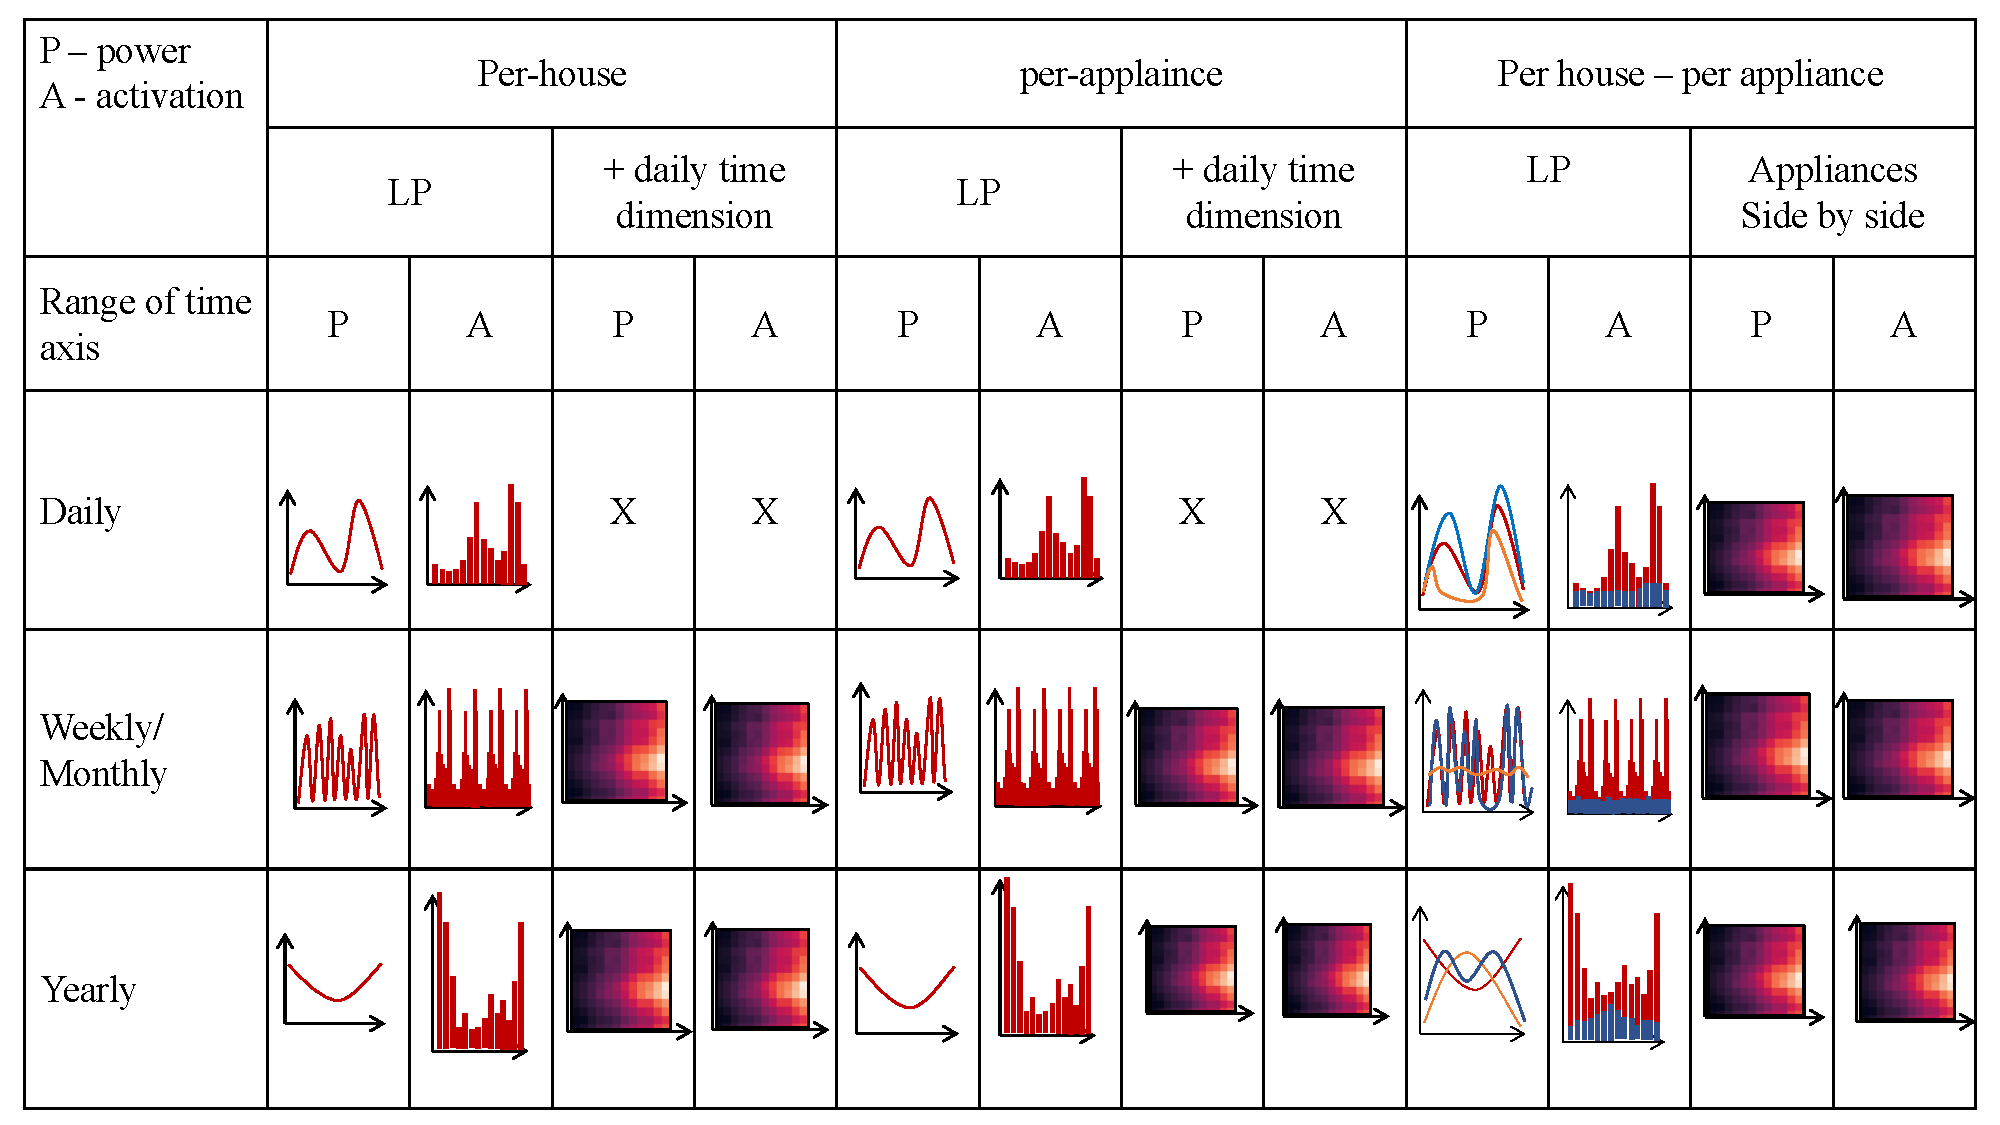
\includegraphics[width=0.9\textwidth]{Figures/profile_sketches/slide14.pdf}
  \caption{Table of combinations}
  \label{fig:map_fig}
\end{sidewaysfigure}

Table \ref{fig:map_fig}, uses features from the previous Section \ref{sec:subfeatures}. 
In general, Table \ref{fig:map_fig} is formatted in a way that features from columns (time range) are
used in the x-axis of a plot, and rows (consumption data) are used in the y or z-axis of a plot. 

The column of Table \ref{fig:map_fig} presents the time domain.
"Daily" means that the LP presents average usage for one day and "Weekly" means it presents usage for a week.
To be clear, for one to construct a decent daily profile, one needs a few weeks of data. 
The same goes for yearly profiles, in that case, one needs many years' worth of data. 

The top row of Table \ref{fig:map_fig} is composed of 3 main groups. 
The first group focuses on per-building energy consumption.
The second group examines the energy consumption of each appliance in a house separately.
The third group analyses all appliances in a building.

The next row of Table \ref{fig:map_fig} is further divided into two groups. 
First is the LP group which presents the given usage unit on the y-axis and time on the x-axis. 
Next is an LP with an additional time axis. 
In this case, we present the given usage unit on the z-axis and then time on the x and y-axis.
Here, the second-time dimension can be anything from a week to a year.
In the case of the per-building, the subgroup includes appliances instead of time. 
An example of this is Figure \ref{fig:heatmap_all_appl}.

The last row presents the usage unit, that is power (P) or the number of activations (A).

In cases where the feature combination does not make sense, it is marked with an X.

\subsection{Mapping References to the Table of Profiles}

To find useful LPs, references from the related work Section \ref{sec:related_work} must be mapped.

\begin{table}[H]
  \centering
	\caption{Table presents previously mentioned LPs}
	\label{tab:contributions}
  \centering
	\begin{tabular}{|c|cccc|cccc|cccc|}
	\hline
	\begin{tabular}[c]{@{}l@{}} P - power \\A - activation\end{tabular}                                                   & \multicolumn{4}{c|}{\textbf{Per-building}}                                                                                               & \multicolumn{4}{c|}{\textbf{Per-appliance}}                                                                                           & \multicolumn{4}{c|}{\begin{tabular}[c]{@{}c@{}}\textbf{Per-building}\\ \textbf{per-appliance}\end{tabular}}                                                         \\ \cline{2-13}
																 & \multicolumn{2}{c|}{\textbf{LP}}                         & \multicolumn{2}{c|}{\begin{tabular}[c]{@{}c@{}} \textbf{+ daily}\\\textbf{dim.}\end{tabular}} & \multicolumn{2}{c|}{\textbf{LP}}                         & \multicolumn{2}{c|}{\begin{tabular}[c]{@{}c@{}} \textbf{+ daily}\\\textbf{dim.} \end{tabular}} & \multicolumn{2}{c|}{\textbf{LP}}                               & \multicolumn{2}{c|}{\begin{tabular}[c]{@{}c@{}}\textbf{Appl.}\\ \textbf{by side}\end{tabular}} \\ \hline
	\begin{tabular}[c]{@{}l@{}} \textbf{Interval} \end{tabular} & \multicolumn{1}{c|}{\textbf{P}} & \multicolumn{1}{c|}{\textbf{A}} & \multicolumn{1}{c|}{\textbf{P}}                         & {\textbf{A}}                         & \multicolumn{1}{c|}{\textbf{P}} & \multicolumn{1}{c|}{\textbf{A}} & \multicolumn{1}{c|}{\textbf{P}}                         & {\textbf{A}}                         & \multicolumn{1}{c|}{\textbf{P}}    & \multicolumn{1}{c|}{\textbf{A}}    & \multicolumn{1}{c|}{\textbf{P}}                               & {\textbf{A}}                               \\ \hline
	\textbf{Daily}                                                        & \multicolumn{1}{c|}{\begin{tabular}[c]{@{}c@{}} \citeyear*{UKDALE} \\ \citeyear*{Chuan2014} \\ \citeyear*{Csoknyai2019} \\ \citeyear*{H0} \\ \citeyear*{KAVOUSIAN2013184} \\ \citeyear*{CAPASSO1994} \\ \citeyear*{WALKER1985} \\ \citeyear*{GERBEC2005} \\ \citeyear*{Gao2018} \\ \citeyear*{Jeong2021} \\ \citeyear*{Joana2012} \\ \citeyear*{DER_heatmap_profile} \end{tabular}}  & \multicolumn{1}{c|}{}  & \multicolumn{1}{c|}{X}  &  X  & \multicolumn{1}{c|}{\begin{tabular}[c]{@{}l@{}} \citeyear*{NILMAD2019} \\ \citeyear*{NILMAD22019} \\ \citeyear*{Issi2018} \\ \citeyear*{NILMAD2021} \\ \citeyear*{Castangia2021} \\ \citeyear*{occupancy2013}	\end{tabular}}  & \multicolumn{1}{c|}{\citeyear*{UKDALE}}  & \multicolumn{1}{c|}{X}   &  \multicolumn{1}{c|}{X}   & \multicolumn{1}{c|}{\begin{tabular}[c]{@{}l@{}} \citeyear*{Chuan2014} \\ \citeyear*{CAPASSO1994} \\ \citeyear*{Gao2018} 	\end{tabular}}   & \multicolumn{1}{c|}{\citeyear*{UKDALE}}     & \multicolumn{1}{c|}{}      &    \\ \hline
	\begin{tabular}[c]{@{}l@{}}\textbf{Weekly/} \\ \textbf{Monthly/} \end{tabular}    & \multicolumn{1}{c|}{\begin{tabular}[c]{@{}c@{}} \citeyear*{Csoknyai2019} \\ \citeyear*{H0} \\ \citeyear*{KAVOUSIAN2013184} \end{tabular}}  & \multicolumn{1}{c|}{}  & \multicolumn{1}{c|}{\begin{tabular}[c]{@{}l@{}} \citeyear*{2D_year_day_LP} \\ \citeyear*{Park2019} \\ \citeyear*{DER_heatmap_profile} \end{tabular}}                            &                           & \multicolumn{1}{c|}{}  & \multicolumn{1}{c|}{\citeyear*{per_appliance_per_building}}  & \multicolumn{1}{c|}{}                          &                           & \multicolumn{1}{c|}{\citeyear*{weekly_per_appliance_LP}}    & \multicolumn{1}{c|}{\citeyear*{per_appliance_per_building}}     & \multicolumn{1}{c|}{}                                &                                 \\ \hline
	\textbf{Yearly}                                                       & \multicolumn{1}{c|}{\begin{tabular}[c]{@{}c@{}} \citeyear*{Csoknyai2019} \\ \citeyear*{H0} \\ \citeyear*{KAVOUSIAN2013184} \end{tabular}}  & \multicolumn{1}{c|}{}  & \multicolumn{1}{c|}{}                          &                           & \multicolumn{1}{c|}{}  & \multicolumn{1}{c|}{}  & \multicolumn{1}{c|}{}                          &                           & \multicolumn{1}{c|}{}     & \multicolumn{1}{c|}{}     & \multicolumn{1}{c|}{}                                &                                 \\ \hline
	\end{tabular}
\end{table}

As can be seen from Table \ref{tab:contributions}, most of the work (14 publications) has been done with standard daily LPs with
per-building power usage such as Figure \ref{fig:daily_power_profile}. 
Quite a lot of work (6 publications), has been done with per-appliance daily power profiles.
A few publications were based on weekly and yearly LPs and a few used two-dimensional time and power presentations.
Only one publication found used activation and time-based histogram such as 
shown in Figure \ref{fig:daily_act_profile}. During the research we focused on publications
from minority classes, meaning not all existing publications for standard LPs are included. 
The purpose of Table \ref{tab:contributions} is to present missing scientific contributions and patterns of publications.  

\newcommand{\tabVar}{\textbf{+ daily} \\ \textbf{dim}  }

\subsection{Mapping Use-Cases to the Table of Profiles}

Table \ref{tab:use_cases} includes arranged publications from the use-cases Section \ref{sec:use-cases}. 
A similar pattern emerged as in Table \ref{tab:contributions}. 

\begin{table}[H]
  \centering
	\caption{Table presents references mentioned in use-cases Chapter}
	\label{tab:use_cases}
	\begin{tabular}{|c|cccc|cccc|cccc|}
	\hline
	  \begin{tabular}[c]{@{}l@{}} P -  power \\A - activation \end{tabular} &
	  \multicolumn{4}{c|}{\textbf{Per-building}} &
	  \multicolumn{4}{c|}{\textbf{Per-appliance}} &
	  \multicolumn{4}{c|}{\begin{tabular}[c]{@{}c@{}}\textbf{Per-building}\\ \textbf{per-appliance}\end{tabular}} \\  \cline{2-13}
	  &
	  \multicolumn{2}{c|}{\textbf{LP}} &
	  \multicolumn{2}{c|}{\begin{tabular}[c]{@{}c@{}} \tabVar \end{tabular}} &
	  \multicolumn{2}{c|}{\textbf{LP}} &
	  \multicolumn{2}{c|}{\begin{tabular}[c]{@{}c@{}} \tabVar \end{tabular}} &
	  \multicolumn{2}{c|}{\textbf{LP}} &
	  \multicolumn{2}{c|}{\begin{tabular}[c]{@{}c@{}}\textbf{Appl}\\ \textbf{by side}\end{tabular}} \\ \hline
	\begin{tabular}[c]{@{}l@{}}\textbf{Interval}\end{tabular} &
	  \multicolumn{1}{c|}{\textbf{P}} &
	  \multicolumn{1}{c|}{\textbf{A}} &
	  \multicolumn{1}{c|}{\textbf{P}} &
	  {\textbf{A}} &
	  \multicolumn{1}{c|}{\textbf{P}} &
	  \multicolumn{1}{c|}{\textbf{A}} &
	  \multicolumn{1}{c|}{\textbf{P}} &
	  {\textbf{A}} &
	  \multicolumn{1}{c|}{\textbf{P}} &
	  \multicolumn{1}{c|}{\textbf{A}} &
	  \multicolumn{1}{c|}{\textbf{P}} &
	  {\textbf{A}} \\ \hline
	\textbf{Daily} &
	  \multicolumn{1}{c|}{\begin{tabular}[c]{@{}c@{}} \citeyear*{energy_saving1} \\ \citeyear*{energy_saving3} \\ \citeyear*{EV2020} \\ \citeyear*{energyStealing2018} \\ \citeyear*{shift2015} \\ \citeyear*{optimiseCostShift2015} \\ \citeyear*{controll2014} \end{tabular}} &
	  \multicolumn{1}{c|}{} &
	  \multicolumn{1}{c|}{X} &
    X
	   &
	  \multicolumn{1}{c|}{\begin{tabular}[c]{@{}c@{}} \citeyear*{EV2020} \\ \citeyear*{elder1} \\ \citeyear*{elder2} \\   \citeyear*{occupancy2013}	  \end{tabular}} &
	  \multicolumn{1}{c|}{} &
	  \multicolumn{1}{c|}{X} &
    X
	   &
	  \multicolumn{1}{c|}{\citeyear*{Chuan2014}	 } &
	  \multicolumn{1}{c|}{} &
	  \multicolumn{1}{c|}{} &
	   \\ \hline
	\begin{tabular}[c]{@{}l@{}}\textbf{Weekly/} \\ \textbf{Monthly/} \end{tabular} &
	  \multicolumn{1}{c|}{\begin{tabular}[c]{@{}c@{}} \citeyear*{energy_saving3} \\ \citeyear*{KAVOUSIAN2013184}  \end{tabular}} &
	  \multicolumn{1}{c|}{} &
	  \multicolumn{1}{c|}{} &
	   &
	  \multicolumn{1}{c|}{} &
	  \multicolumn{1}{c|}{} &
	  \multicolumn{1}{c|}{} &
	   &
	  \multicolumn{1}{c|}{} &
	  \multicolumn{1}{c|}{} &
	  \multicolumn{1}{c|}{} &
	   \\ \hline
	\textbf{Yearly} &
	  \multicolumn{1}{c|}{\begin{tabular}[c]{@{}c@{}}\citeyear*{energy_saving3}\end{tabular}} &
	  \multicolumn{1}{c|}{} &
	  \multicolumn{1}{c|}{} &
	   &
	  \multicolumn{1}{c|}{} &
	  \multicolumn{1}{c|}{} &
	  \multicolumn{1}{c|}{} &
	   &
	  \multicolumn{1}{c|}{} &
	  \multicolumn{1}{c|}{} &
	  \multicolumn{1}{c|}{} &
	   \\ \hline
	\end{tabular}
\end{table}

\subsection{Table of Use-Case Groups}

The Table \ref{tab:groups} presents same publications as Table \ref{tab:use_cases},
but only group names are shown. 
The groups are the main use cases from Section \ref{sec:use-cases} and use-case tree in Chapter \ref{sec:use_cases_tree}.


\begin{itemize}
  \item ZEB - zero energy buildings
  \item DR - demand response
  \item AD - anomaly detection
  \item EC - elderly care
  \item X - unfeasible
\end{itemize}

The Table \ref{tab:groups} indicates how groups are arranged.
Where anomaly detection and elderly care are dominating in the per-appliance part of the table,
zero energy buildings and demand response are dominating in a per-building part of the table. 

\begin{table}[H]
  \centering
  \caption{Table presents references mentioned in use-cases Chapter}
	\label{tab:groups}
    %\begin{adjustbox}{width=1.0\textwidth,center=\textwidth} 
        \begin{tabular}{|c|cccc|cccc|cccc|}
            \hline
             \begin{tabular}[c]{@{}l@{}} P -  power \\A - activation \end{tabular} &
              \multicolumn{4}{c|}{\textbf{Per-building}} &
              \multicolumn{4}{c|}{\textbf{Per-appliance}} &
              \multicolumn{4}{c|}{\begin{tabular}[c]{@{}c@{}}\textbf{Per-building}\\ \textbf{per-appliance}\end{tabular}} \\ \cline{2-13} 
             &
              \multicolumn{2}{c|}{\textbf{LP}} &
              \multicolumn{2}{c|}{\begin{tabular}[c]{@{}c@{}}\textbf{+ daily} \\ \textbf{dim}\end{tabular}} &
              \multicolumn{2}{c|}{\textbf{LP}} &
              \multicolumn{2}{c|}{\begin{tabular}[c]{@{}c@{}} \tabVar \end{tabular}} &
              \multicolumn{2}{c|}{\textbf{LP}} &
              \multicolumn{2}{c|}{\begin{tabular}[c]{@{}c@{}}\textbf{Appl}\\ \textbf{by side}\end{tabular}} \\ \hline
            \begin{tabular}[c]{@{}l@{}}\textbf{Interval}\end{tabular} &
              \multicolumn{1}{c|}{\textbf{P}} &
              \multicolumn{1}{c|}{\textbf{A}} &
              \multicolumn{1}{c|}{\textbf{P}} &
              {\textbf{A}} &
              \multicolumn{1}{c|}{\textbf{P}} &
              \multicolumn{1}{c|}{\textbf{A}} &
              \multicolumn{1}{c|}{\textbf{P}} &
              {\textbf{A}} &
              \multicolumn{1}{c|}{\textbf{P}} &
              \multicolumn{1}{c|}{\textbf{A}} &
              \multicolumn{1}{c|}{\textbf{P}} &
              {\textbf{A}} \\ \hline
            \textbf{Daily} &
              \multicolumn{1}{c|}{\begin{tabular}[c]{@{}c@{}}ZEB,\\ EC\end{tabular}} &
              \multicolumn{1}{c|}{} &
              \multicolumn{1}{c|}{X} &
              X
               &
              \multicolumn{1}{c|}{\begin{tabular}[c]{@{}c@{}}AD,\\ EC,\\ ZEB\end{tabular}} &
              \multicolumn{1}{c|}{} &
              \multicolumn{1}{c|}{X} &
              X
               &
              \multicolumn{1}{c|}{DR} &
              \multicolumn{1}{c|}{} &
              \multicolumn{1}{c|}{} &
               \\ \hline
            \begin{tabular}[c]{@{}l@{}}\textbf{Weekly/} \\ \textbf{Monthly/} \end{tabular} &
              \multicolumn{1}{c|}{ZEB} &
              \multicolumn{1}{c|}{} &
              \multicolumn{1}{c|}{} &
               &
              \multicolumn{1}{c|}{} &
              \multicolumn{1}{c|}{} &
              \multicolumn{1}{c|}{} &
               &
              \multicolumn{1}{c|}{} &
              \multicolumn{1}{c|}{} &
              \multicolumn{1}{c|}{} &
               \\ \hline
            \textbf{Yearly} &
              \multicolumn{1}{c|}{ZEB} &
              \multicolumn{1}{c|}{} &
              \multicolumn{1}{c|}{} &
               &
              \multicolumn{1}{c|}{} &
              \multicolumn{1}{c|}{} &
              \multicolumn{1}{c|}{} &
               &
              \multicolumn{1}{c|}{} &
              \multicolumn{1}{c|}{} &
              \multicolumn{1}{c|}{} &
               \\ \hline
            \end{tabular}
    %\end{adjustbox} 
    \end{table}

    
The figures listed above clearly depict the void not filled by publications. 
Although they may not be published, they still have a possible use case. 
In Table \ref{tab:groups_proposed} empty spaces are filled 
with possible use-cases for given LPs. 

\begin{table}[H]
    \centering
    \caption{Proposed use-cases for profiles}
    \label{tab:groups_proposed}
    \begin{adjustbox}{width=1.0\textwidth,center=\textwidth} 
    \begin{tabular}{|c|cccc|cccc|cccc|}
    \hline
    \begin{tabular}[c]{@{}l@{}}P - power \\A - activation\end{tabular} &
      \multicolumn{4}{c|}{\textbf{Per-building}} &
      \multicolumn{4}{c|}{\textbf{Per-appliance}} &
      \multicolumn{4}{c|}{\begin{tabular}[c]{@{}c@{}}\textbf{Per-building}\\ \textbf{per-appliance}\end{tabular}} \\ \cline{2-13} 
     &
      \multicolumn{2}{c|}{\textbf{LP}} &
      \multicolumn{2}{c|}{\begin{tabular}[c]{@{}c@{}}\textbf{+ daily} \\ \textbf{dim}\end{tabular}} &
      \multicolumn{2}{c|}{\textbf{LP}} &
      \multicolumn{2}{c|}{\begin{tabular}[c]{@{}c@{}} \tabVar \end{tabular}} &
      \multicolumn{2}{c|}{\textbf{LP}} &
      \multicolumn{2}{c|}{\begin{tabular}[c]{@{}c@{}}\textbf{Appl}\\ \textbf{by side}\end{tabular}} \\ \hline
    \begin{tabular}[c]{@{}l@{}}\textbf{Interval}\end{tabular} &
      \multicolumn{1}{c|}{\textbf{P}} &
      \multicolumn{1}{c|}{\textbf{A}} &
      \multicolumn{1}{c|}{\textbf{P}} &
      {\textbf{A}} &
      \multicolumn{1}{c|}{\textbf{P}} &
      \multicolumn{1}{c|}{\textbf{A}} &
      \multicolumn{1}{c|}{\textbf{P}} &
      {\textbf{A}} &
      \multicolumn{1}{c|}{\textbf{P}} &
      \multicolumn{1}{c|}{\textbf{A}} &
      \multicolumn{1}{c|}{\textbf{P}} &
      {\textbf{A}} \\ \hline
    \textbf{Daily} &
      \multicolumn{1}{c|}{\begin{tabular}[c]{@{}c@{}}AD,\\ ZEB,\\ DR,\end{tabular}} &
      \multicolumn{1}{c|}{\begin{tabular}[c]{@{}c@{}}AD,\\ ZEB,\\ DR,\end{tabular}} &
      \multicolumn{1}{c|}{X} &
      X &
      \multicolumn{1}{c|}{\begin{tabular}[c]{@{}c@{}}AD,\\ EC,\\ ZEB,\\ DR\end{tabular}} &
      \multicolumn{1}{c|}{\begin{tabular}[c]{@{}c@{}}AD,\\ EC,\\ ZEB,\\ DR\end{tabular}} &
      \multicolumn{1}{c|}{\begin{tabular}[c]{@{}c@{}} X \end{tabular}} &
      \begin{tabular}[c]{@{}c@{}} X \end{tabular} &
      \multicolumn{1}{c|}{\begin{tabular}[c]{@{}c@{}}AD,\\ EC,\\ ZEB,\\ DR\end{tabular}} &
      \multicolumn{1}{c|}{\begin{tabular}[c]{@{}c@{}}AD,\\ EC,\\ ZEB,\\ DR\end{tabular}} &
      \multicolumn{1}{c|}{\begin{tabular}[c]{@{}c@{}}AD,\\ EC,\\ ZEB,\\ DR\end{tabular}} &
      \begin{tabular}[c]{@{}c@{}}AD,\\ EC,\\ ZEB,\\ DR\end{tabular} \\ \hline
    \begin{tabular}[c]{@{}l@{}}\textbf{Weekly/} \\ \textbf{Monthly/} \end{tabular} &
      \multicolumn{1}{c|}{\begin{tabular}[c]{@{}c@{}}AD,\\ ZEB,\\ DR\end{tabular}} &
      \multicolumn{1}{c|}{\begin{tabular}[c]{@{}c@{}}AD,\\ ZEB,\\ DR,\end{tabular}} &
      \multicolumn{1}{c|}{\begin{tabular}[c]{@{}c@{}}ZEB,\\ DR \end{tabular}} &
      \multicolumn{1}{c|}{\begin{tabular}[c]{@{}c@{}}ZEB,\\ DR \end{tabular}} &
      \multicolumn{1}{c|}{\begin{tabular}[c]{@{}c@{}}AD,\\ ZEB,\\ DR\end{tabular}} &
      \multicolumn{1}{c|}{\begin{tabular}[c]{@{}c@{}}AD,\\ ZEB,\\ DR\end{tabular}} &
      \multicolumn{1}{c|}{\begin{tabular}[c]{@{}c@{}}AD,\\ ZEB,\\ DR\end{tabular}} &
      \begin{tabular}[c]{@{}c@{}}AD,\\ ZEB,\\ DR\end{tabular} &
      \multicolumn{1}{c|}{\begin{tabular}[c]{@{}c@{}}AD,\\ ZEB,\\ DR\end{tabular}} &
      \multicolumn{1}{c|}{\begin{tabular}[c]{@{}c@{}}AD,\\ ZEB,\\ DR\end{tabular}} &
      \multicolumn{1}{c|}{\begin{tabular}[c]{@{}c@{}}AD,\\ ZEB,\\ DR\end{tabular}} &
      \begin{tabular}[c]{@{}c@{}}AD,\\ ZEB,\\ DR\end{tabular} \\ \hline
    \textbf{Yearly} &
      \multicolumn{1}{c|}{\begin{tabular}[c]{@{}c@{}}ZEB,\\ DR\end{tabular}} &
      \multicolumn{1}{c|}{\begin{tabular}[c]{@{}c@{}}ZEB,\\ DR\end{tabular}} &
      \multicolumn{1}{c|}{\begin{tabular}[c]{@{}c@{}}ZEB,\\ DR\end{tabular}} &
      \multicolumn{1}{c|}{\begin{tabular}[c]{@{}c@{}}ZEB,\\ DR\end{tabular}} &
      \multicolumn{1}{c|}{\begin{tabular}[c]{@{}c@{}}AD,\\ ZEB,\\ DR\end{tabular}} &
      \multicolumn{1}{c|}{\begin{tabular}[c]{@{}c@{}}AD,\\ ZEB,\\ DR\end{tabular}} &
      \multicolumn{1}{c|}{\begin{tabular}[c]{@{}c@{}}ZEB,\\ DR\end{tabular}} &
      \multicolumn{1}{c|}{\begin{tabular}[c]{@{}c@{}}ZEB,\\ DR\end{tabular}} &
      \multicolumn{1}{c|}{\begin{tabular}[c]{@{}c@{}}ZEB,\\ DR\end{tabular}} &
      \multicolumn{1}{c|}{\begin{tabular}[c]{@{}c@{}}AD,\\ ZEB,\\ DR\end{tabular}} &
      \multicolumn{1}{c|}{\begin{tabular}[c]{@{}c@{}}AD,\\ ZEB,\\ DR\end{tabular}} &
      \begin{tabular}[c]{@{}c@{}}AD,\\ ZEB,\\ DR\end{tabular} \\ \hline
    \end{tabular}
    \end{adjustbox}
\end{table}

\subsection{Table of LP Potentials} \label{subsec:potential}

Some combinations are indeed illogical and again others are less useful in a practical sense.
The next Table \ref{tab:classified_profiles} will try to rate the utilization potential of the profiles based on two characteristics. 
First is how well data is presented to the user,
meaning that the LP is clear about what it is presenting.
The second is the effectiveness when being used in an algorithm, or in other words, how well data is presented to a machine. 

These characteristics can not be easily measured,
but it is possible to extract them based on the pattern of publications.
To do that, we have to make two assumptions.
The first one would be, that the larger the number of publications, the larger the effect of presenting the data to a human.
The second would be, that the larger the number of use cases, the better the effectiveness of presenting the data to a machine.
Using these two assumptions, we propose the following table. 
The Table has four possible classes. 

\begin{outline} 
\1 1 - The LP satisfies both assumptions and has a high utility rate and was already researched (very useful, but with low research potential). 
\1 2 - The LP satisfies only one of the above-mentioned assumptions (has mid-research potential).
\1 3 - The LP does not suffice any of the above-mentioned assumptions and was not yet researched or practically used (high research potential, could be hard to utilize).
\1 X - The LP is inexplicable (does not make any sense).
\end{outline}

\begin{table}[H]
    \centering
    \caption{Proposed classification of profiles}
    \label{tab:classified_profiles}
    \begin{tabular}{|c|cccc|cccc|cccc|}
    \hline
     \begin{tabular}[c]{@{}l@{}}P - power \\A - activation\end{tabular} &
      \multicolumn{4}{c|}{\textbf{Per-building}} &
      \multicolumn{4}{c|}{\textbf{Per-appliance}} &
      \multicolumn{4}{c|}{\begin{tabular}[c]{@{}c@{}}\textbf{Per-building}\\ \textbf{per-appliance}\end{tabular}} \\ \cline{2-13} 
     &
      \multicolumn{2}{c|}{\textbf{LP}} &
      \multicolumn{2}{c|}{\begin{tabular}[c]{@{}c@{}}\textbf{+ daily} \\ \textbf{dim}\end{tabular}} &
      \multicolumn{2}{c|}{\textbf{LP}} &
      \multicolumn{2}{c|}{\begin{tabular}[c]{@{}c@{}} \tabVar \end{tabular}} &
      \multicolumn{2}{c|}{\textbf{LP}} &
      \multicolumn{2}{c|}{\begin{tabular}[c]{@{}c@{}}\textbf{Appl}\\ \textbf{by side}\end{tabular}} \\ \hline
    \begin{tabular}[c]{@{}l@{}}\textbf{Interval}\end{tabular} &
      \multicolumn{1}{c|}{\textbf{P}} &
      \multicolumn{1}{c|}{\textbf{A}} &
      \multicolumn{1}{c|}{\textbf{P}} &
      {\textbf{A}} &
      \multicolumn{1}{c|}{\textbf{P}} &
      \multicolumn{1}{c|}{\textbf{A}} &
      \multicolumn{1}{c|}{\textbf{P}} &
      {\textbf{A}} &
      \multicolumn{1}{c|}{\textbf{P}} &
      \multicolumn{1}{c|}{\textbf{A}} &
      \multicolumn{1}{c|}{\textbf{P}} &
      {\textbf{A}} \\ \hline
    \textbf{Daily} &
      \multicolumn{1}{c|}{1} &
      \multicolumn{1}{c|}{3} &
      \multicolumn{1}{c|}{X} &
      X &
      \multicolumn{1}{c|}{1} &
      \multicolumn{1}{c|}{2} &
      \multicolumn{1}{c|}{X} &
      X &
      \multicolumn{1}{c|}{1} &
      \multicolumn{1}{c|}{2} &
      \multicolumn{1}{c|}{3} &
      3 \\ \hline
    \begin{tabular}[c]{@{}l@{}}\textbf{Weekly/} \\ \textbf{Monthly/} \end{tabular} &
      \multicolumn{1}{c|}{1} &
      \multicolumn{1}{c|}{3} &
      \multicolumn{1}{c|}{2} &
      3 &
      \multicolumn{1}{c|}{3} &
      \multicolumn{1}{c|}{2} &
      \multicolumn{1}{c|}{3} &
      3 &
      \multicolumn{1}{c|}{2} &
      \multicolumn{1}{c|}{2} &
      \multicolumn{1}{c|}{3} &
      3 \\ \hline
    \textbf{Yearly} &
      \multicolumn{1}{c|}{1} &
      \multicolumn{1}{c|}{3} &
      \multicolumn{1}{c|}{3} &
      3 &
      \multicolumn{1}{c|}{3} &
      \multicolumn{1}{c|}{3} &
      \multicolumn{1}{c|}{3} &
      3 &
      \multicolumn{1}{c|}{3} &
      \multicolumn{1}{c|}{3} &
      \multicolumn{1}{c|}{3} &
      3 \\ \hline
    \end{tabular}
\end{table}

\subsection{Table of Possible Future Research Directions}

To find future research directions we must look into profiles that were least researched,
such profiles are marked with the number 3 on Table \ref{tab:classified_profiles}.
Some profiles were not researched because they may not present data as well and some were simply overlooked. 
This is why we have built the following Table \ref{tab:future_rd}.
The Table was populated as follows:

\begin{outline} 
\1 (1) - The LP has high potential. 
\1 (2) - The LP has mid-potential.
\1 Empty - The LP has low potential or was already researched.
\1 X - LP is inexplicable
\end{outline}

The process of evaluation was a bit complicated, but it can be summed down to the following rules.

If the LP was used as a power profile, can it be used as an activation profile?
Here, we must use common sense.
For example. If we follow this rule for per-building power LPs, it 
turns out that activation LPs are not as useful since they are based on per-appliance LPs.
In other words, to build per-building activation LPs we need per-appliance (sub-meter) data anyway.
That is why we have assigned them to the second class.

The second rule was applied to 3D profiles.
In the case where one dimension was commonly used, it is probably worth investigating it with a combination of additional dimensions. 

Following these rules, Table  \ref{tab:future_rd} was constructed.


\begin{table}[H]
    \centering
    \caption{Possible future research contributions}
    \label{tab:future_rd}
    \begin{tabular}{|c|cccc|cccc|cccc|}
    \hline
     \begin{tabular}[c]{@{}l@{}}P - power \\A - activation\end{tabular} &
      \multicolumn{4}{c|}{\textbf{\textbf{Per-building}}} &
      \multicolumn{4}{c|}{\textbf{Per-appliance}} &
      \multicolumn{4}{c|}{\begin{tabular}[c]{@{}c@{}}\textbf{Per-building}\\ \textbf{per-appliance}\end{tabular}} \\ \cline{2-13} 
     &
      \multicolumn{2}{c|}{\textbf{LP}} &
      \multicolumn{2}{c|}{\begin{tabular}[c]{@{}c@{}}\textbf{+ daily} \\ \textbf{dim}\end{tabular}} &
      \multicolumn{2}{c|}{\textbf{LP}} &
      \multicolumn{2}{c|}{\begin{tabular}[c]{@{}c@{}} \tabVar \end{tabular}} &
      \multicolumn{2}{c|}{\textbf{LP}} &
      \multicolumn{2}{c|}{\begin{tabular}[c]{@{}c@{}}\textbf{Appl}\\ \textbf{by side}\end{tabular}} \\ \hline
    \begin{tabular}[c]{@{}l@{}}\textbf{Interval}\end{tabular} &
      \multicolumn{1}{c|}{\textbf{P}} &
      \multicolumn{1}{c|}{\textbf{A}} &
      \multicolumn{1}{c|}{\textbf{P}} &
      {\textbf{A}} &
      \multicolumn{1}{c|}{\textbf{P}} &
      \multicolumn{1}{c|}{\textbf{A}} &
      \multicolumn{1}{c|}{\textbf{P}} &
      {\textbf{A}} &
      \multicolumn{1}{c|}{\textbf{P}} &
      \multicolumn{1}{c|}{\textbf{A}} &
      \multicolumn{1}{c|}{\textbf{P}} &
      {\textbf{A}} \\ \hline
    \textbf{Daily} &
      \multicolumn{1}{c|}{} &
      \multicolumn{1}{c|}{(2)} &
      \multicolumn{1}{c|}{X} &
      X
       &
      \multicolumn{1}{c|}{} &
      \multicolumn{1}{c|}{} &
      \multicolumn{1}{c|}{X} &
      X
       &
      \multicolumn{1}{c|}{} &
      \multicolumn{1}{c|}{} &
      \multicolumn{1}{c|}{(1)} &
      (1) \\ \hline
    \begin{tabular}[c]{@{}l@{}}\textbf{Weekly/} \\ \textbf{Monthly/} \end{tabular} &
      \multicolumn{1}{c|}{} &
      \multicolumn{1}{c|}{(2)} &
      \multicolumn{1}{c|}{} &
      (1) &
      \multicolumn{1}{c|}{(1)} &
      \multicolumn{1}{c|}{} &
      \multicolumn{1}{c|}{(1)} &
      (1) &
      \multicolumn{1}{c|}{} &
      \multicolumn{1}{c|}{} &
      \multicolumn{1}{c|}{(2)} &
      (2) \\ \hline
    \textbf{Yearly} &
      \multicolumn{1}{c|}{} &
      \multicolumn{1}{c|}{} &
      \multicolumn{1}{c|}{} &
       &
      \multicolumn{1}{c|}{(2)} &
      \multicolumn{1}{c|}{(2)} &
      \multicolumn{1}{c|}{} &
       &
      \multicolumn{1}{c|}{} &
      \multicolumn{1}{c|}{} &
      \multicolumn{1}{c|}{(2)} &
      (2) \\ \hline
    \end{tabular}
\end{table}

Table \ref{tab:future_rd} presents the possible future research directions. 
While some LPs have mid-research potential according to our rules, they are still worth investigating. 
In science, it often happens that use-cases change over time and research that seemed inapplicable suddenly finds its place.

We will focus on profiles with high research potential and use the number of activations as a unit of measure.
When the aforementioned parameters are applied, 
the result is Table \ref{tab:our_rd}.

\begin{table}[H]
    \centering
    \caption{LPs to be pursued}
    \label{tab:our_rd}
    \begin{tabular}{|c|cccc|cccc|cccc|}
    \hline
     \begin{tabular}[c]{@{}l@{}} P - power \\A - activation\end{tabular} &
      \multicolumn{4}{c|}{\textbf{Per-building}} &
      \multicolumn{4}{c|}{\textbf{Per-appliance}} &
      \multicolumn{4}{c|}{\begin{tabular}[c]{@{}c@{}}\textbf{Per-building}\\ \textbf{per-appliance}\end{tabular}} \\ \cline{2-13} 
     &
      \multicolumn{2}{c|}{\textbf{LP}} &
      \multicolumn{2}{c|}{\begin{tabular}[c]{@{}c@{}}\textbf{+ daily} \\ \textbf{dim}\end{tabular}} &
      \multicolumn{2}{c|}{\textbf{LP}} &
      \multicolumn{2}{c|}{\begin{tabular}[c]{@{}c@{}} \tabVar \end{tabular}} &
      \multicolumn{2}{c|}{\textbf{LP}} &
      \multicolumn{2}{c|}{\begin{tabular}[c]{@{}c@{}}\textbf{Appl}\\ \textbf{by side}\end{tabular}} \\ \hline
    \begin{tabular}[c]{@{}l@{}}\textbf{Interval}\end{tabular} &
      \multicolumn{1}{c|}{\textbf{P}} &
      \multicolumn{1}{c|}{\textbf{A}} &
      \multicolumn{1}{c|}{\textbf{P}} &
      {\textbf{A}} &
      \multicolumn{1}{c|}{\textbf{P}} &
      \multicolumn{1}{c|}{\textbf{A}} &
      \multicolumn{1}{c|}{\textbf{P}} &
      {\textbf{A}} &
      \multicolumn{1}{c|}{\textbf{P}} &
      \multicolumn{1}{c|}{\textbf{A}} &
      \multicolumn{1}{c|}{\textbf{P}} &
      {\textbf{A}} \\ \hline
    \textbf{Daily} &
      \multicolumn{1}{c|}{} &
      \multicolumn{1}{c|}{} &
      \multicolumn{1}{c|}{X} &
      X
      &
      \multicolumn{1}{c|}{} &
      \multicolumn{1}{c|}{} &
      \multicolumn{1}{c|}{X} &
      X
      &
      \multicolumn{1}{c|}{} &
      \multicolumn{1}{c|}{} &
      \multicolumn{1}{c|}{} &
      (1) \\ \hline
    \begin{tabular}[c]{@{}l@{}}\textbf{Weekly/} \\ \textbf{Monthly/} \end{tabular} &
      \multicolumn{1}{c|}{} &
      \multicolumn{1}{c|}{} &
      \multicolumn{1}{c|}{} &
      (1) &
      \multicolumn{1}{c|}{} &
      \multicolumn{1}{c|}{} &
      \multicolumn{1}{c|}{} &
      (1) &
      \multicolumn{1}{c|}{} &
      \multicolumn{1}{c|}{} &
      \multicolumn{1}{c|}{} &
       \\ \hline
    \textbf{Yearly} &
      \multicolumn{1}{c|}{} &
      \multicolumn{1}{c|}{} &
      \multicolumn{1}{c|}{} &
       &
      \multicolumn{1}{c|}{} &
      \multicolumn{1}{c|}{} &
      \multicolumn{1}{c|}{} &
       &
      \multicolumn{1}{c|}{} &
      \multicolumn{1}{c|}{} &
      \multicolumn{1}{c|}{} &
       \\ \hline
    \end{tabular}
    \end{table}

The profiles shown in Table \ref{tab:our_rd} are our direction of research.
In the next part of the thesis, we will try to utilize and present these LPs.
This will be done as follows.
In Chapter \ref{chapter5} we will use
\begin{itemize}
  \item Per-building daily-weekly LP
  \item Per-appliance daily-weekly LP
\end{itemize}
with a t-SNE neighboring algorithm to find how they are related in high dimensional space.
In Chapter \ref{chapter6} we will use
\begin{itemize}
  \item Per-building Per-appliance daily LPs with appliances side by side
\end{itemize}
To build assisted living system for the elderly.

